\section{Experimental Details \& Further Discussion}\label{sec:appendix_experimental_details}

\subsection{Relational Games (Section \ref{ssec:relgames})}\label{ssec:appendxi_relgames}

\subsubsection*{Experimental details}

\textbf{Dataset details.} The Relational Games benchmark datasets consists of $36 \times 36 \times 3$ RGB images depicting a $3 \times 3$ grid of objects which satisfy a particular visual relationship. The task is to identify whether a given relationship holds or not. The set of objects consists of simple geometric shapes. Examples of each task are presented in~\Cref{fig:relgames_examples}. For example, in the \texttt{occurs} task, one object is present in the top row and three in the bottom row, and the task is to determine whether the object in the top row occurs (i.e., is among) the objects in the bottom row. The most difficult task in the benchmark is the \texttt{match pattern} task, where the grid contains a triplet of objects in the top row and another triplet of objects in the bottom row. Each triplet satisfies some relationship (e.g., ABC, ABA, ABB, or AAB), and the task is to determine whether the relation in the first triplet is the same as the relation in the second triplet. The difficulty in solving this task is that it requires parsing a second-order relation (a relation between relations). We remark that composing relational attention modules naturally captures this kind of hierarchical relations: the first relational attention operation produces objects representing relational information and the second would compute relations between those relations (i.e., second-order relations).

\begin{figure}
    \centering
    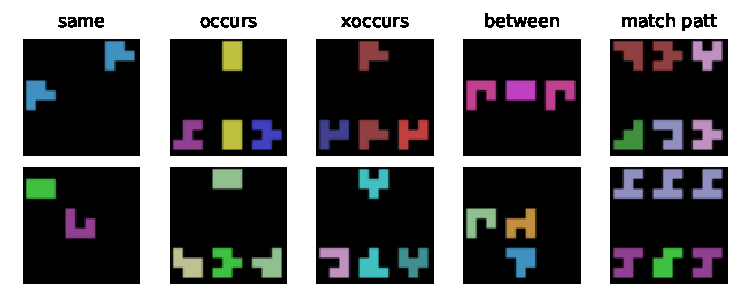
\includegraphics[width=0.8\textwidth]{figs/experiments/relgames/relational_games_tasks.pdf}
    \caption{Examples of different tasks in the Relational Games benchmark. Each column corresponds to a different task in the benchmark. The top row is an example of a positive instance and the bottom row is an example of a negative instance.}\label{fig:relgames_examples}
\end{figure}

\textbf{Model architectures.} We use a Vision-Transformer-type architecture where the input image is split up into patches, flattened, and passed through the sequence model with added learned positional embeddings. We use average pooling at the end and pass through an MLP to produce the final prediction. We use a patch size of $12 \times 12$ which separates objects according to the grid structure. We note that in more general visual relational reasoning tasks where there isn't this type of grid structure, it would be appropriate to combine our approach with an object-discovery module such as Slot Attention~\citep{locatelloObjectCentricLearningSlot2020}.

We use 2-layer models. The \textit{DAT} models use $\dmodel = 128$, $\dff = 256$. One set of Transformer baselines uses the same, while another is larger with $\dmodel = 144$, $\dff = 288$. All models use SwiGLU ``activation'', dropout rate = 0.1, and pre-LayerNormalization. For the \textit{DAT} models, we use positional symbols as the symbol assignment mechanism. The composition of sensory and relational attention heads are depicted in the figure. In~\Cref{fig:relgames_learning_curves}, we use symmetric relations (i.e., imposing that $\Wqrel = \Wkrel$). Below, we also explore the effect of this inductive bias, evaluating variants without the symmetry constraint.

\textbf{Training details.} For each task and model, we evaluated learning curves by varying the training set size and training the model until convergence, then evaluating on a hold-out test set. For four out of five of the tasks, we evaluate learning curves within the range of $250$ to $2,500$ samples, in increments of $250$. For the more difficult \texttt{match pattern}, the range is from $5,000$ to $25,000$ in increments of $5,000$. The ranges were chosen based on the difficulty of the different tasks in order to identify the right ``resolution''. When evaluating learning curves, each training set is sampled randomly from the full dataset. For each task, model, and training set size, we repeat the experiment 5 times with different random seeds to compute approximate confidence intervals (accounting for randomness in sampling the dataset and random initialization). We use an Adam optimizer with a learning rate of $0.001$, $\beta_1 = 0.9, \beta_2 = 0.99$, and a batch size of $512$. We train for 50 epochs.

\subsubsection*{Further Discussion, Exploration, \& Ablations}

\textbf{Comparison to previous relational architectures.} Previous research has explored relational learning in synthetic settings, proposing various architectures with relational inductive biases. Here, we compare \textit{DAT} to three such architectures: PrediNet~\citep{shanahanExplicitlyRelationalNeurala}, CoRelNet~\citep{kergNeuralArchitectureInductive2022}, and Abstractor~\citep{altabaa2024abstractors}. Unlike \textit{DAT}, these architectures use subtractive rather than additive relational inductive biases, imposing constraints on the types of learnable representations to improve relational learning efficiency. As a result, they are not general-purpose architectures and cannot be applied to broader domains such as language modeling. Nonetheless, it is useful to compare \textit{DAT} against those architectures to explore the trade-offs of strong inductive biases and evaluate \textit{DAT} in comparison to alternative approaches to relational learning. \Cref{fig:relgames_baselines} shows learning curves comparing \textit{DAT} against those baselines. \textit{DAT} performs competitively with previous relational architectures, generally outperforming PrediNet and Abstractor, while performing marginally worse than CoRelNet. It is relevant to note that CoRelNet incorporates strong task-specific inductive biases, and was partially designed with this benchmark in mind.

\begin{figure}[h]
    \centering
    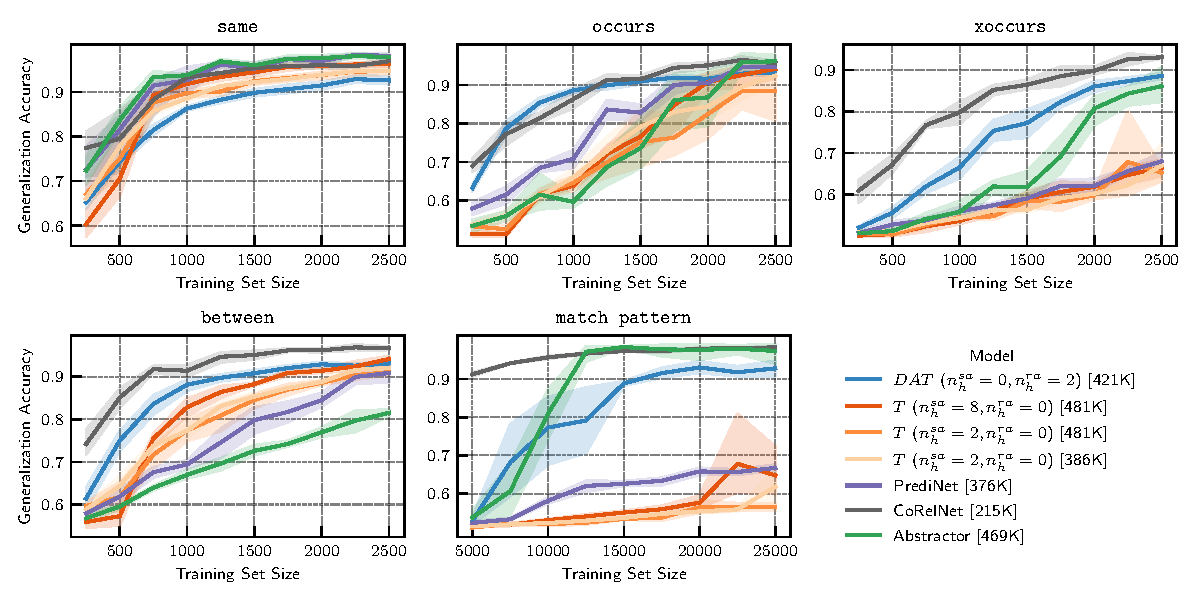
\includegraphics[width=\textwidth]{figs/experiments/relgames/relgames_learning_curves_baseline_comparisons.pdf}
    \caption{Learning curves on the Relational Games benchmark, comparing \textit{DAT} against previously-proposed relational architectures. \textit{DAT} performs competitively with previous relational architectures.}\label{fig:relgames_baselines}
\end{figure}

\textbf{Ablation over symmetry.} We performed an ablation over the \textit{symmetry} inductive bias in the relations computed in relational attention. Our implementation exposes an argument which controls whether the relation $r(x, y) = (\iiprod{\Wqrell{\ell}}{\Wkrell{\ell}})_{\ell \in [d_r]} \in \reals^{d_r}$ modeled in relational attention is constrained to be symmetric by setting $\Wqrell{\ell} = \Wkrell{\ell}$. Indeed, we find symmetry to be a useful inductive bias in this task.~\Cref{fig:relgames_symmetry_ablation} depicts learning curves for the two configurations of \textit{DAT} comparing symmetric RA against asymmetric RA. We find that symmetry results in faster learning curves for both configurations.

\begin{figure}[h]
    \centering
    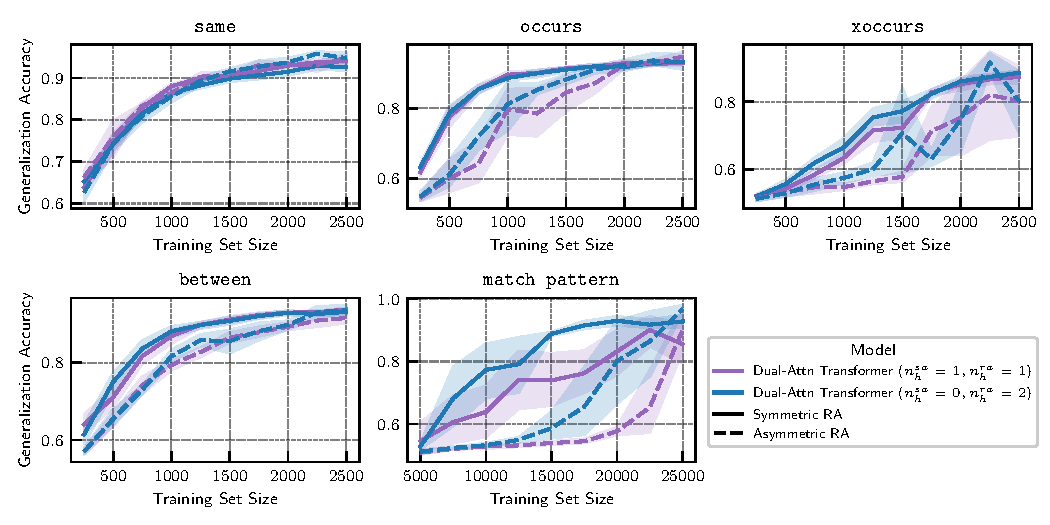
\includegraphics[width=\textwidth]{figs/experiments/relgames/relgames_learning_curves_symmetry_ablation.pdf}
    \caption{An ablation of the effect of symmetry in relational attention in the relational games experiments.}\label{fig:relgames_symmetry_ablation}
\end{figure}

\subsection{Mathematical Problem-Solving (Section \ref{ssec:math})}\label{ssec:appendix_math}

\subsubsection*{Experimental details}

\textbf{Dataset details.} \citet{saxtonAnalyzingMathematicalReasoning2019} propose a benchmark to assess neural models' ability to perform mathematical reasoning. The dataset consists of a suite of tasks in free-form textual input/output format. The tasks cover several topics in mathematics, including arithmetic, algebra, and calculus. For each task, the authors programmatically generate $2 \times 10^6$ training examples and $10^4$ validation examples. Questions have a maximum length of 160 characters and answers have a maximum length of 30 characters.

\aanote{TODO -- add examples of input-output sequences for tested tasks?}

\textbf{Model architectures.} We use an encoder-decoder architecture for this experiment, treating it as a sequence-to-sequence task. We use character-level encoding with a common alphabet of size 85 containing small and upper case letters, digits 0-9, and symbols (e.g., \texttt{*, /, +, -}). We vary the number of layers to explore how performance scales with model size in \textit{DAT} compared to standard Transformers. Each encode/decoder block uses ReLU activation, dropout rate = 0.1, and post-normalization. We use $\dmodel = 128, \dff = 256$ for the \textit{DAT} models and $\dmodel = 144, \dff = 288$ in the Transformer models to control for parameter count and give the Transformer an advantage in the evaluation. Sinusoidal positional embeddings are used as the positional encoding method. For all models, the total number of attention heads (across self-attention and relational attention) is $8$. For the Transformer model, there are only self-attention heads: $\nhsa = 8$ for both the encoder and decoder. For \textit{DAT}, we evaluated two configurations for the composition of head types, one with $\nhsa = \nhra = 4$ in the encoder and $\nhsa = 8, \nhra = 0$ in the decoder (i.e., standard Transformer Decoder), and one with $\nhsa = 4 = \nhra = 4$ in the encoder and $\nhsa = 4 = \nhra = 4$ in the decoder. The number of cross-attention heads in the decoder is $8$ in all cases. No symmetry constraint is made on relational attention. Position-relative symbols are used as the symbol assignment mechanism, and the symbol library is shared across all layers in both the encoder and decoder.

\textbf{Training Details.} Each model is trained on each task for 50 epochs. We use the Adam optimizer with $\beta_1 = 0.9, \beta_2 = 0.995$, a learning rate of $6 \times 10^{-4}$, and a batch size of 128. We evaluate and track the per-character accuracy over the course of training. We repeat this process 5 times for each combination of model and task with different random seeds to compute approximate confidence intervals.

\subsubsection*{Further Discussion, Exploration, \& Ablations}

\Cref{tab:math_full_results} reports the full set of results obtained for this experiment, including certain configurations omitted from the figure in the main text.

\begin{table}
    \resizebox{\textwidth}{!}{%
    \begin{tabular}{l|l|cc}
\toprule
Task & Model &  Accuracy \\
\midrule
\multirow{7}{*}{$\texttt{algebra\_\_linear\_1d}$} & Transformer [692K] &                    62.5\% \\
                                 & $DAT$ [783K] &                    66.5\% \\
                                 & Transformer [871K] &                    64.0\% \\
                                 & $DAT$ [1.09M] &                    76.6\% \\
                                 & Transformer [1.3M] &                    64.3\% \\
                                 & $DAT$ [1.43M] &                    74.7\% \\
                                 & Transformer [1.7M] &                    50.9\% \\
\cline{1-3}
\multirow{7}{*}{$\texttt{algebra\_\_sequence\_next\_term}$} & Transformer [692K] &                    91.1\% \\
                                 & $DAT$ [783K] &                    91.6\% \\
                                 & Transformer [871K] &                    91.4\% \\
                                 & $DAT$ [1.09M] &                    97.3\% \\
                                 & Transformer [1.3M] &                    96.9\% \\
                                 & $DAT$ [1.43M] &                        -- \\
                                 & Transformer [1.7M] &                    82.6\% \\
\cline{1-3}
\multirow{7}{*}{$\texttt{calculus\_\_differentiate}$} & Transformer [692K] &                    99.9\% \\
                                 & $DAT$ [783K] &                   100.0\% \\
                                 & Transformer [871K] &                    99.9\% \\
                                 & $DAT$ [1.09M] &                        -- \\
                                 & Transformer [1.3M] &                    99.9\% \\
                                 & $DAT$ [1.43M] &                   100.0\% \\
                                 & Transformer [1.7M] &                   100.0\% \\
\cline{1-3}
\multirow{7}{*}{$\texttt{polynomials\_\_add}$} & Transformer [692K] &                    83.3\% \\
                                 & $DAT$ [783K] &                    85.6\% \\
                                 & Transformer [871K] &                    84.5\% \\
                                 & $DAT$ [1.09M] &                    87.9\% \\
                                 & Transformer [1.3M] &                    86.9\% \\
                                 & $DAT$ [1.43M] &                    88.7\% \\
                                 & Transformer [1.7M] &                    87.3\% \\
\cline{1-3}
\multirow{7}{*}{$\texttt{polynomials\_\_expand}$} & Transformer [692K] &                    74.0\% \\
                                 & $DAT$ [783K] &                    77.8\% \\
                                 & Transformer [871K] &                    74.1\% \\
                                 & $DAT$ [1.09M] &                        -- \\
                                 & Transformer [1.3M] &                        -- \\
                                 & $DAT$ [1.43M] &                    92.2\% \\
                                 & Transformer [1.7M] &                    87.2\% \\
\bottomrule
\end{tabular}

    }
    %\vskip 10pt
    \caption{Full results of mathematical problem-solving experiments. For each task, this table shows the mean test character-level accuracy $\pm$ the standard error of mean for each model configuration.}\label{tab:math_full_results}
\end{table}


% This benchmark contains two validation splits: an interpolation split and an extrapolation split. The interpolation split is generated by the same procedure as the training split. The extrapolation split is generated with different parameters to make the task more difficult. We refer to the original reference for more details~\citep{saxtonAnalyzingMathematicalReasoning2019}.~\Cref{fig:math_training_curves_interpolation} in the main text depicts the interpolation validation accuracy.~\Cref{fig:math_training_curves_extrapolation} depicts the extrapolation validation accuracy over the course of training. For completeness, we also show the training accuracy in~\Cref{fig:math_training_curves_trainacc}.

% \begin{figure}
%     \centering
%     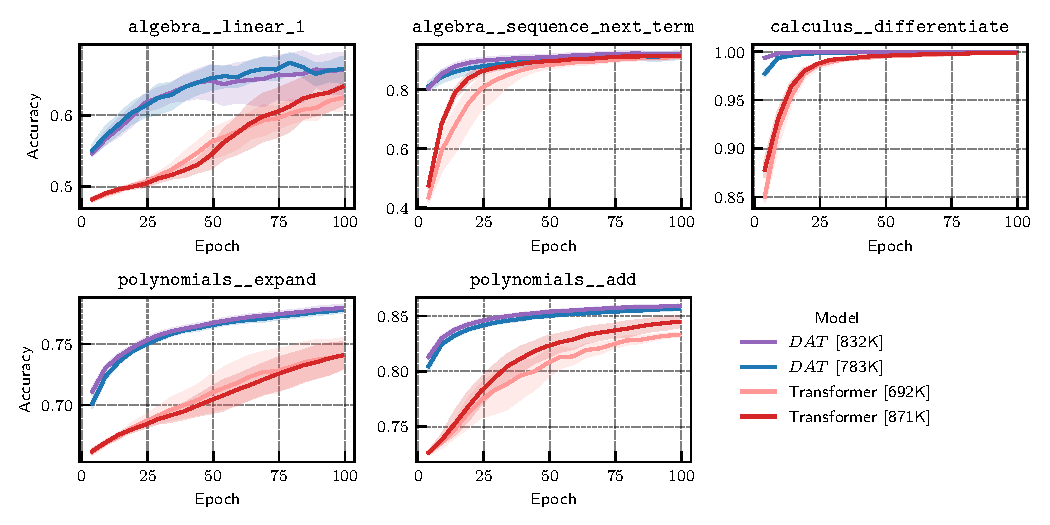
\includegraphics[width=\textwidth]{figs/experiments/math/math_training_curves_extrapolation.pdf}
%     \caption{Extrapolation validation accuracy over the course of training for mathematical problem-solving tasks.}\label{fig:math_training_curves_extrapolation}
% \end{figure}

% \begin{figure}
%     \centering
%     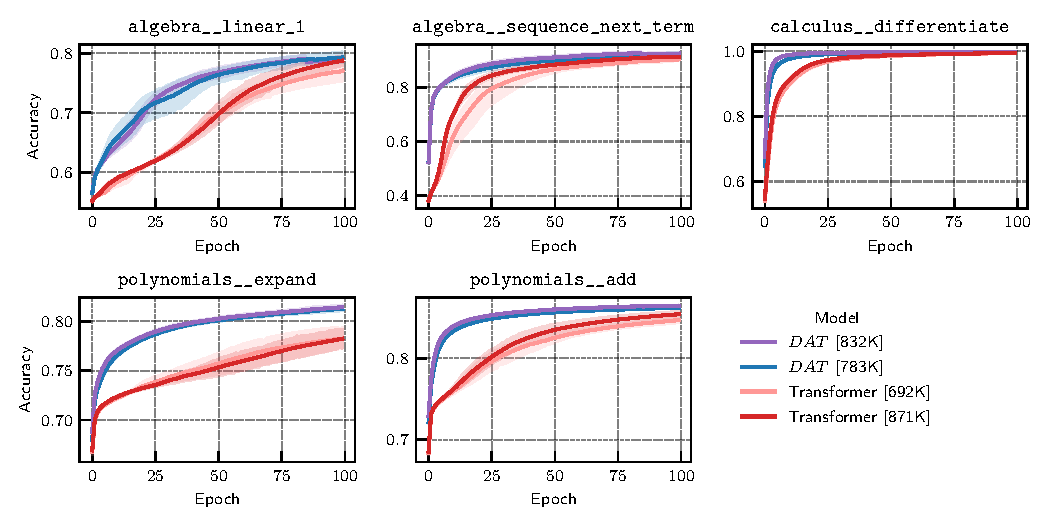
\includegraphics[width=\textwidth]{figs/experiments/math/math_training_curves_trainacc.pdf}
%     \caption{Training accuracy over the course of training for mathematical problem-solving tasks.}\label{fig:math_training_curves_trainacc}
% \end{figure}


\subsection{Visual Processing (Section \ref{ssec:vision})}\label{ssec:appendix_vision}

\subsubsection*{Experimental details}

\textbf{Dataset details.} In this set of experiments, we use the CIFAR-10 and CIFAR-100 datasets~\citep{cifar_dataset} which are datasets of labeled small images. The CIFAR-10 dataset consists of $60,000$ $32 \times 32$ RGB images, evenly split across 10 classes. The CIFAR-100 dataset consists of $60,000$ RGB images of the same size, evenly split across 100 classes.

\textbf{Model architectures.} We use a \textit{ViT}-style architecture~\citep{dosovitskiyImageWorth16x162020}. RGB images are divided into $4 \times 4$ patches, flattened, linearly embedded into a vector, and fed through an Encoder. We use average pooling followed by an MLP to produce the final prediction. We evaluate 8-layer models with $\dmodel = \dff = 384$, GeLU activation, Pre-LayerNormalization, and no dropout. The \textit{ViT} model has $\nhsa = 12$ standard self-attention heads, while the \textit{DAT} model uses both sensory and relational heads, with an even split $\nhsa = \nhra = 6$. In the main text, we use symmetric relations $\bm{r}_{ij}$ with the intuition that visual processing involves symmetric attribute-similarity relations. We also carried out experiments with asymmetric relations and discuss the results below. In \textit{DAT}, we use position-relative symbols as the symbol assignment mechanism. Further, we use Grouped Query Attention~\citep{ainslie-etal-2023-gqa} in \textit{DAT} to reduce the parameter count to account for the added parameters in relational attention.

\textbf{Training Details.} We train for 100 epochs. We use the Adam optimizer with a learning rate schedule consisting of a gradual warmup to $10^{-3}$ in the first 5 epochs, followed by a cosine rate decay down to $10^{-5}$. We use the hyperparameters $\beta_1 = 0.9, \beta_2 = 0.999$, and weight decay of $5 \cdot 10^{-5}$. We normalize the images channel-wise such that pixels have mean zero and unit standard deviation. In the results reported in~\Cref{tab:cifar_results} in the main text, we use random cropping, MixUp~\citep{zhang2018mixup}, and CutMix~\citep{yun2019cutmix} as data augmentation techniques during training. We also report results using AutoAugment~\citep{cubuk2019autoaugmentlearningaugmentationpolicies} below.

\subsubsection*{Further Discussion, Exploration, \& Ablations}

\textbf{Effect of symmetry in $\bm{r}_{ij}$.} In the main text, \Cref{tab:cifar_results} reports \textit{DAT} results with symmetric relations $\bm{r}_{ij}$ by imposing $\Wqrel = \Wkrel$. Here, we explore the effect of this choice. \Cref{tab:cifar_results_symmetry_ablation} compares \textit{DAT} models with and without the symmetry constraint. We find no significant difference in performance. Though, we note the smaller parameter count in the symmetric variant.

\begin{table}
    \resizebox{\textwidth}{!}{
    \begin{tabular}{l|l|cccccc|c}
\toprule
Dataset & Model & Parameter Count & \# Layers & $d_{\text{model}}$ & $n_h^{sa}$ & $n_h^{ra}$ & Symmetric $\bm{r}_{ij}$ & Accuracy\\
\midrule
\multirow{3}{*}{CIFAR-10} & \textit{ViT} & 7.1M & 8 & 384 & 12 & 0 & NA &  $86.4 \pm 0.1\%$ \\\cline{2-9}
          & \multirow{2}{*}{\textit{ViDAT}} & 6.0M & 8 & 384 & 6  & 6 & Yes &  $89.7 \pm 0.1\%$ \\
          &       & 6.6M & 8 & 384 & 6  & 6 & No &  $89.5 \pm 0.1\%$ \\
\midrule
\multirow{3}{*}{CIFAR-100} & \textit{ViT} & 7.2M & 8 & 384 & 12 & 0 & NA &  $68.8 \pm 0.2\%$ \\\cline{2-9}
          & \multirow{2}{*}{\textit{ViDAT}} & 6.1M & 8 & 384 & 6  & 6 & Yes &  $70.5 \pm 0.1\%$ \\
          &       & 6.7M & 8 & 384 & 6  & 6 & No &  $70.5 \pm 0.1\%$ \\
\bottomrule
\end{tabular}

    }
    %\vskip5pt
    \caption{Ablation over symmetry of $\bm{r}_{ij}$ in relational attention for image recognition experiments.}\label{tab:cifar_results_symmetry_ablation}
\end{table}

\textbf{Alternative data augmentation.} In the main text, we use random cropping, MixUp, and CutMix data augmentation during training. Here, we report results on an alternative data augmentation technique: AutoAugment~\citep{cubuk2019autoaugmentlearningaugmentationpolicies}. AutoAugment is an optimized set of data augmentation policies, found through a data-dependent automatic search procedure. At each mini-batch, a random sub-policy is chosen which consists of image processing operations such as translation, rotation, or shearing. \Cref{tab:cifar_results_autoaugment} reports results using this data augmentation procedure. We continue to find that \textit{ViDAT} outperforms the standard \textit{ViT} model.

\begin{table}
    \begin{tabular}{l|l|ccccc|c}
\toprule
Dataset & Model & Parameter Count & \# Layers & $d_{\text{model}}$ & $n_h^{sa}$ & $n_h^{ra}$ & Accuracy \\
\midrule
\multirow{2}{*}{CIFAR-10} & \textit{ViT} & 7.1M & 8 & 384 & 12 & 0 &  $89.5 \pm 0.1\%$ \\
          & \textit{ViDAT} & 6.0M & 8 & 384 & 6  & 6 &  $\bm{91.7 \pm 0.1\%}$ \\
\midrule
\multirow{2}{*}{CIFAR-100} & \textit{ViT} & 7.2M & 8 & 384 & 12 & 0 &  $68.2 \pm 0.1\%$ \\
          & \textit{ViDAT} & 6.1M & 8 & 384 & 6  & 6 &  $\bm{70.9 \pm 0.1\%}$ \\
\bottomrule
\end{tabular}

    %\vskip5pt
    \caption{Classification accuracy on CIFAR-10 and CIFAR-100 with AutoAugment data augmentation during training. Each training configuration is repeated 10 times with different random seeds; we report the mean accuracy $\pm$ the standard error of mean. \textit{DAT} continues to outperform the standard Vision Transformer.}\label{tab:cifar_results_autoaugment}
\end{table}

\subsection{Language Modeling (Section \ref{ssec:fineweb})}\label{ssec:appendix_fineweb}

\subsubsection*{Experimental details}

\textbf{Dataset details.} The FineWeb-Edu~\citep{lozhkov2024fineweb-edu} dataset is a curated dataset of text data. It is generated by filtering the large-scale FineWeb dataset for LLM pre-training~\citep{penedo2024finewebdatasetsdecantingweb} using an educational quality classifier trained on annotations generated by LLama3-70B-instruct. FineWeb-Edu has been shown to outperform FineWeb on several benchmarks, demonstrating the importance of data \textit{quality}. We train our language models on a random subset of 10 billion tokens of FineWeb-Edu.

\textbf{Model Architectures.} We use a Decoder-only architecture, with causal attention for autoregressive language modeling. We vary model size to explore the scaling properties of \textit{DAT} with respect to both model size and data size, comparing to the scaling properties of standard Transformers. Our architectural hyperparameters follow common choices at different model scales, based on scaling analyses performed for Transformers~\citep{penedo2024finewebdatasetsdecantingweb}. We explore 3 model scales: 350M ($\dmodel = 1024, n_h = 16, L = 24$), 750M ($\dmodel = 1536, n_h = 24, L = 24$), and 1.3B ($\dmodel = 2048, n_h = 32, L = 24$) parameters. We use $\dff = 4 \cdot \dmodel$, GeLU activation, RoPE positional encoding, no bias, no dropout, and Pre-LayerNormalization. We use the GPT2 tokenizer~\citep{radford2019language}. We use symbolic attention as the symbol assignment mechanism, with the number of symbols in the symbol library scaling with model size: 1024 symbols and 8 heads for the 350M and 750M scale models, and 2048 symbols with 16 heads for the 1.3B scale model. We also increase the relation dimension with model size. We don't impose a symmetry constraint, with the intuition that linguistic relations can be asymmetric. We use Grouped Query Attention in the \textit{DAT} models to reduce parameter count to account for the added parameters in relational attention, making them smaller overall compared to the Transformer baselines at each parameter scale.

\textbf{Training Details.} We train for 10B Tokens, with each batch containing $524,288$ tokens, split into context windows of $1,024$ tokens. We use gradient accumulation to fit micro-batches into memory. We use the AdamW optimizer with a maximum learning rate of $6 \times 10^{-4}$ and minimum learning rate of $6 \times 10^{-5}$, first linearly warming up over the first 715 steps, then decaying back down with a cosine schedule. We use $\beta_1 = 0.9, \beta_2 = 0.95$ and a weight decay of $0.1$. We also use gradient clipping to unit norm.

\subsubsection*{Further Discussion, Exploration, \& Ablations}

\Cref{fig:fineweb_param_data} in the main text depicts the scaling properties of a \textit{DAT} language model with respect to model size and data size compared to a standard Transformer. Here, we provide a few additional representations of the results. \Cref{tab:fineweb_results} reports the end-of-training validation perplexity of the different models. 

\Cref{fig:fineweb_training_curves} depicts training curves for the different model scales. We observe a power law scaling of the validation loss with respect to number of training tokens. This matches the neural scaling laws \citep{kaplan2020scalinglawsneurallanguage}, which suggest that validation loss ought to scale roughly as $d^{-\alpha}$ where $d$ is the amount of training data and the exponent $\alpha$ is a constant that depends on model architecture, training details, etc.

\begin{table}[h]
    \centering
    \caption{End-of-training validation perplexity in language modeling on FineWeb-Edu dataset.}\label{tab:fineweb_results}
    % \begin{tabular}{@{}l|ccccccc|c@{}}
\begin{tabular}{@{}lcc|cccccc|c@{}}
    \toprule
    Model        & Param count   & \# Tokens &$\dmodel$&$\nlayers$& $\nhsa$  & $\nhra$ & $d_r$ & $n_{kv}^{h}$ & Perplexity $\downarrow$ \\ \midrule\hline
    Transformer  & 353M   & 10B       & 1024    & 24       & 16       & -        & -     & -           & 16.94     \\
    \textit{DAT} & 343M   & 10B       & 1024    & 24       & 8        & 8        & 8    & 4           & 16.26     \\
    \textit{DAT} & 343M   & 10B       & 1024    & 24       & 8        & 8        & 32    & 4           & 16.14     \\
    \textit{DAT} & 343M   & 10B       & 1024    & 24       & 8        & 8        & 64    & 4           & 16.09     \\
    % \textit{DAT} & 368M   & 10B       & 1024    & 24       & 8        & 8        & 8   & 8           & 15.97     \\\midrule
    Transformer  & 1.31B  & 10B       & 2048    & 24       & 32       & -        & -     & -           & 13.63     \\
    \textit{DAT} & 1.27B  & 10B       & 2048    & 24       & 16       & 16       & 64    & 8           & 13.44     \\
    \textit{DAT} & 1.37B  & 10B       & 2048    & 24       & 16       & 16       & 64    & -          & 13.43     \\ \bottomrule
    % Model / Param count   &$\dmodel$&$\nlayers$& $\nhsa$  & $\nhra$ & $n_r$ & $n_{kv}^{h}$ & Perplexity $\downarrow$ \\ \midrule\hline
    % Transformer - 353M   & 1024    & 24       & 16       & -        & -     & -           & 16.944     \\
    % \textit{DAT} - 343M  & 1024    & 24       & 8        & 8        & 32    & 4           & 16.258     \\
    % \textit{DAT} - 368M  & 1024    & 24       & 8        & 8        & 32    & 8           & 15.969     \\\midrule
    % Transformer - 1.31B  & 2048    & 24       & 32       & -        & -     & -           & 13.630     \\
    % \textit{DAT} - 1.27B & 2048    & 24       & 16       & 16       & 64    & 8           & 13.440     \\
    % \textit{DAT} - 1.37B & 2048    & 24       & 16       & 16       & 64    & 16          & 13.426     \\ \bottomrule
\end{tabular}%
    % }
    % & $n_s$ 
    % & -     
    % & 1024  
    % & 1024  
    % & -     
    % & 512   
    % & 2048  
\end{table}

\begin{figure}[h]
    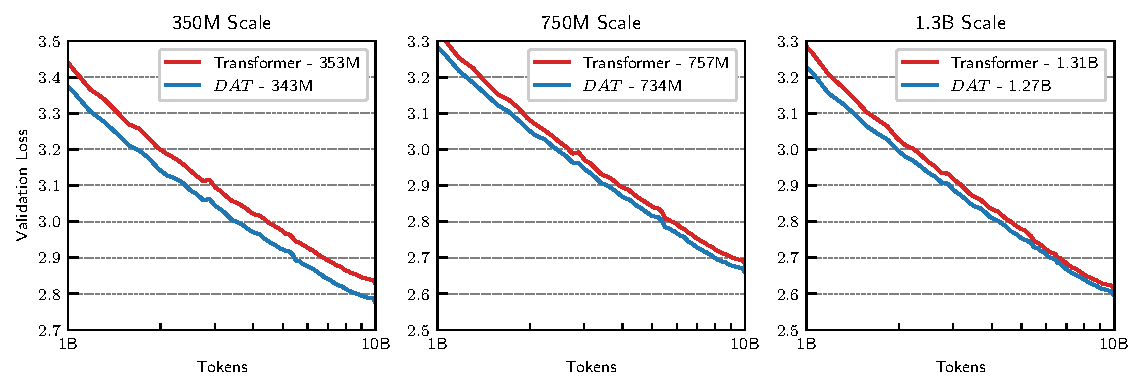
\includegraphics[width=\textwidth]{figs/experiments/fineweb/valloss_logtok.pdf}
    \caption{Validation loss on a logarithmic scale to examine data scaling laws. Dual Attention Transformer language models obey similar scaling laws as standard Transformers with respect to the amount of training data, while consistently achieving smaller loss at multiple model scales.}\label{fig:fineweb_training_curves}
\end{figure}


% \begin{figure}
%     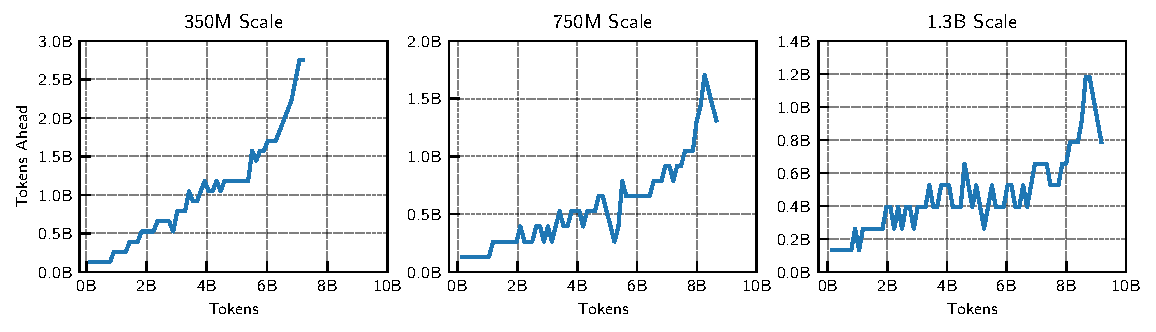
\includegraphics[width=\textwidth]{figs/experiments/fineweb/tokens_ahead.pdf}
% \end{figure}

% \begin{figure}
%     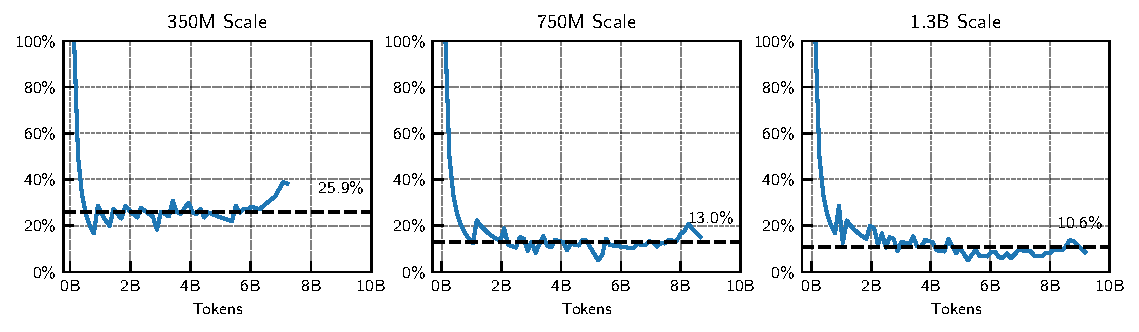
\includegraphics[width=\textwidth]{figs/experiments/fineweb/tokens_ahead_percent.pdf}
%     \caption{A way to contextualize improvement in terms of scaling laws. Number of tokens that \textit{DAT} is ahead of the Transformer over the course of training. In other words, how many tokens fewer the \textit{DAT} model needs to train to reach the same perplexity as the Transformer model. Formally, let $\mathtt{TOK}_{M}(p)$ be the number of tokens needed to reach a perplexity of $p$ for a model $M$, and let $\mathtt{PPL}_{M}(t)$ be the perplexity reached at token $t$ for a model $M$. We plot $(\mathtt{TOK}_{\mathrm{Transformer}}(\mathtt{PPL}_{\text{\textit{DAT}}}(t)) - t) / t$ over the course of training, varying the number of tokens $t$ between 0 and 10B. Dashed line indicates the median percentage of tokens that \textit{DAT} is ahead of the Transformer over the course of training. We see that the amount \textit{DAT} is ahead of the Transformer is relatively consistent throughout training.}\label{fig:fineweb_tokens_ahead_percent}
% \end{figure}



% \subsection{Language Modeling (Section \ref{ssec:tiny_stories})}\label{ssec:appendix_lm}

% \subsubsection*{Experimental details}

% \aanote{TODO -- add samples of generated input? compare across models. add samples of stories from dataset?}

% \textbf{Dataset details.} The Tiny Stories dataset by~\citet{eldanTinyStoriesHowSmall2023} is a language modeling benchmark designed to evaluate small language models. The dataset consists of short stories and is synthetically generated by GPT-3.5 and GPT-4.

% \textbf{Model architectures.} We use a Decoder-only architecture, with causal attention for autoregressive language modeling. We fix the total number of attention heads to be $8$ for all models. For the Transformer model, there are only self-attention heads: $\nhsa = 2$. For \textit{DAT}, we evaluated two configurations for the composition of head types, one with $\nhsa = 6, \nhra = 2$ (more self-attention heads) and one with $\nhsa = \nhra = 4$ (a balanced composition of head types). We experiment with $\dmodel \in \sset{64, 128}$ and number of layers $L \in \sset{4, 5, 6}$. For all models, we use $\dff = 4 \dmodel$, SwiGLU activation in the MLP, RoPE positional encoding, no bias, dropout rate = 0.1, and pre-LayerNormalization. We use weight-tying between the embedding layer and the final prediction layer~\citep{inanTyingWordVectors2016}. For \textit{DAT} models, we perform ablations on the effect of the choice of symbol assignment mechanism and symmetry in relational attention. We train models with position-relative symbols and symbolic attention, as well as models with symmetric and asymmetric relations in relational attention. We use a context size of 512 for all models. Text is tokenized using the Llama SentencePiece tokenizer~\citep{touvronLlamaOpenFoundation2023}, which contains $32,000$ tokens.

% \Cref{fig:tiny_stories_val_loss_curves} in the main text depicts the $\dmodel = 64$ models with varying number of layers $L \in \sset{4, 5, 6}$.~\Cref{fig:tiny_stories_val_loss_curves_d128} shows the loss curves for larger models with $\dmodel = 128$. The \textit{DAT} models use symbolic attention as the symbol assignment mechanism and asymmetric relations in relational attention. Symbolic attention uses $n_s = \texttt{context\_length} = 512$ symbols with 4 heads.

% \textbf{Training Details.} All models are trained with the AdamW optimizer with a constant learning rate of $0.001$ and $\beta_1 = 0.9, \beta_2 = 0.95$. We clip gradients to a norm of 1. Models are trained for $100,000$ iterations. We use a batch size of $128$ with $2$ gradient accumulation steps. Thus, each step trains on $131,072$ tokens.

% \begin{table}
%     \caption{Language Modeling on the Tiny Stories Dataset}\label{tab:tiny_stories_results}
%     
\begin{tabular}{@{}|c|c|c|c|c|c|c|c|@{}}
\toprule
$\dmodel$             & $L$                & $\nhsa$            & $\nhra$            & Symbol Assignment Mechanism                & Symmetric RA & val/loss       & val/perplexity \\
\midrule
\multirow{23}{*}{64}  & \multirow{9}{*}{4} & \multirow{4}{*}{4} & \multirow{4}{*}{4} & \multirow{2}{*}{Position-Relative Symbols} & False        & 1.764          & 5.840          \\
                        &                    &                    &                    &                                            & True         & 1.785          & 5.963          \\ \cline{5-8} 
                        &                    &                    &                    & \multirow{2}{*}{Symbolic Attention}        & False        & \textbf{1.729} & \textbf{5.639} \\
                        &                    &                    &                    &                                            & True         & 1.744          & 5.722          \\ \cline{3-8} 
                        &                    & \multirow{4}{*}{6} & \multirow{4}{*}{2} & \multirow{2}{*}{Position-Relative Symbols} & False        & 1.768          & 5.859          \\
                        &                    &                    &                    &                                            & True         & 1.777          & 5.914          \\ \cline{5-8} 
                        &                    &                    &                    & \multirow{2}{*}{Symbolic Attention}        & False        & 1.740          & 5.697          \\
                        &                    &                    &                    &                                            & True         & 1.745          & 5.727          \\ \cline{3-8} 
                        &                    & 8                  & 0                  & NA                                         & NA           & 1.775          & 5.903          \\ \cline{2-8} 
                        & \multirow{6}{*}{5} & \multirow{2}{*}{4} & \multirow{2}{*}{4} & \multirow{2}{*}{Symbolic Attention}        & False        & \textbf{1.692} & \textbf{5.431} \\
                        &                    &                    &                    &                                            & True         & 1.698          & 5.467          \\ \cline{3-8} 
                        &                    & \multirow{3}{*}{6} & \multirow{3}{*}{2} & Position-Relative Symbols                  & True         & 1.730          & 5.640          \\ \cline{5-8} 
                        &                    &                    &                    & \multirow{2}{*}{Symbolic Attention}        & False        & \textbf{1.692} & \textbf{5.432} \\
                        &                    &                    &                    &                                            & True         & 1.704          & 5.495          \\ \cline{3-8} 
                        &                    & 8                  & 0                  & NA                                         & NA           & 1.730          & 5.640          \\ \cline{2-8} 
                        & \multirow{8}{*}{6} & \multirow{4}{*}{4} & \multirow{4}{*}{4} & \multirow{2}{*}{Position-Relative Symbols} & False        & 1.685          & 5.395          \\
                        &                    &                    &                    &                                            & True         & 1.704          & 5.498          \\ \cline{5-8} 
                        &                    &                    &                    & \multirow{2}{*}{Symbolic Attention}        & False        & \textbf{1.656} & \textbf{5.239} \\
                        &                    &                    &                    &                                            & True         & 1.668          & 5.303          \\ \cline{3-8} 
                        &                    & \multirow{3}{*}{6} & \multirow{3}{*}{2} & Position-Relative Symbols                  & True         & 1.691          & 5.424          \\ \cline{5-8} 
                        &                    &                    &                    & \multirow{2}{*}{Symbolic Attention}        & False        & 1.663          & 5.277          \\
                        &                    &                    &                    &                                            & True         & 1.669          & 5.308          \\ \cline{3-8} 
                        &                    & 8                  & 0                  & NA                                         & NA           & 1.692          & 5.431          \\ \hline
\multirow{10}{*}{128}   & \multirow{5}{*}{4} & \multirow{2}{*}{4} & \multirow{2}{*}{4} & \multirow{2}{*}{Symbolic Attention}        & False        & \textbf{1.411} & \textbf{4.102} \\
                        &                    &                    &                    &                                            & True         & 1.417          & 4.127          \\ \cline{3-8} 
                        &                    & \multirow{2}{*}{6} & \multirow{2}{*}{2} & \multirow{2}{*}{Symbolic Attention}        & False        & 1.412          & 4.105          \\
                        &                    &                    &                    &                                            & True         & 1.415          & 4.118          \\ \cline{3-8} 
                        &                    & 8                  & 0                  & NA                                         & NA           & 1.431          & 4.183          \\ \cline{2-8} 
                        & \multirow{5}{*}{6} & \multirow{2}{*}{4} & \multirow{2}{*}{4} & \multirow{2}{*}{Symbolic Attention}        & False        & \textbf{1.337} & \textbf{3.811} \\
                        &                    &                    &                    &                                            & True         & 1.346          & 3.843          \\ \cline{3-8} 
                        &                    & \multirow{2}{*}{6} & \multirow{2}{*}{2} & \multirow{2}{*}{Symbolic Attention}        & False        & 1.340          & \textbf{3.818} \\
                        &                    &                    &                    &                                            & True         & 1.346          & 3.843          \\ \cline{3-8} 
                        &                    & 8                  & 0                  & NA                                         & NA           & 1.353          & 3.870          \\ \bottomrule
\end{tabular}%
% \end{table}

% \begin{figure}
%     \centering
%     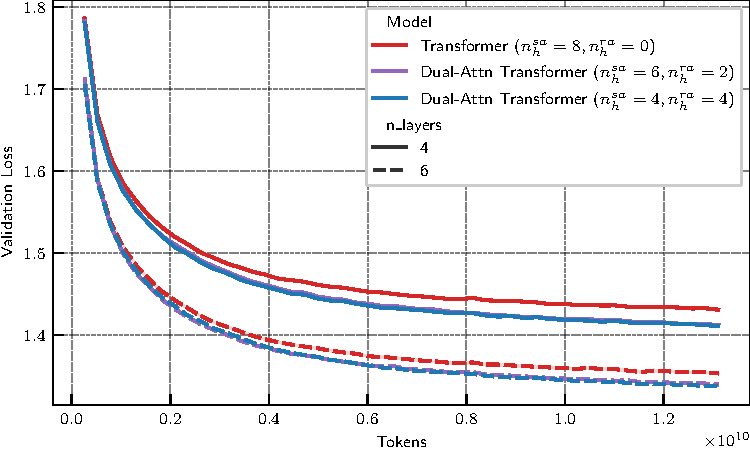
\includegraphics[width=0.5\textwidth]{figs/experiments/tiny_stories/d128L4L6_symattn_asymra.pdf}
%     \caption{Loss curves of \textit{DAT} language models with $\dmodel = 128$.}\label{fig:tiny_stories_val_loss_curves_d128}
% \end{figure}

% \subsubsection*{Further Discussion, Exploration, \& Ablations}

% \begin{figure}
%     \centering
%     \begin{subfigure}[t]{0.45\textwidth}
%         \centering
%         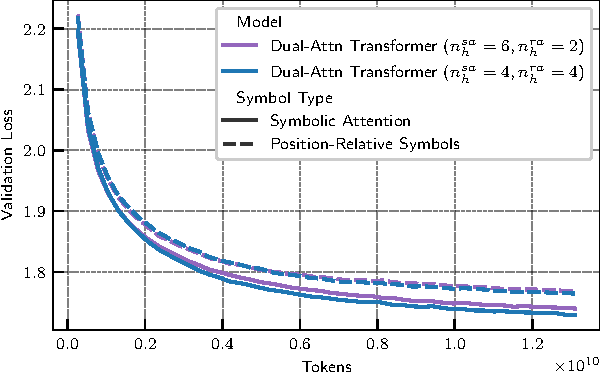
\includegraphics[width=\textwidth]{figs/experiments/tiny_stories/d64L4_ablation_symboltype_asymra.pdf}
%         \caption{$d=64, L=4$, asymmetric RA.}
%     \end{subfigure}
%     \hfill
%     \begin{subfigure}[t]{0.45\textwidth}
%         \centering
%         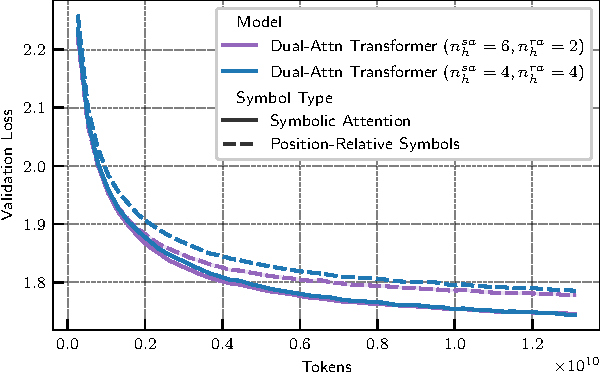
\includegraphics[width=\textwidth]{figs/experiments/tiny_stories/d64L4_ablation_symboltype_symra.pdf}
%         \caption{$d=64, L=4$, symmetric RA.}
%     \end{subfigure}
%     \caption{Ablation of symbol assignment mechanism. Symbolic attention outperforms position-relative symbols.}\label{fig:ablation_symbol_type}
% \end{figure}

% \begin{figure}
%     \centering
%     \begin{subfigure}[t]{0.45\textwidth}
%         \centering
%         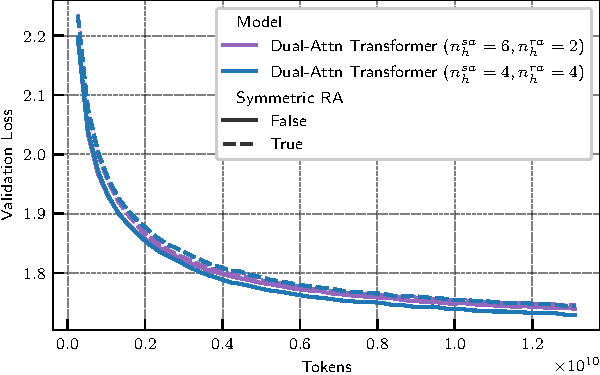
\includegraphics[width=\textwidth]{figs/experiments/tiny_stories/d64L4_ablation_symmetry_symmattn.pdf}
%         \caption{$d = 64, L = 4$, symbolic attention.}
%     \end{subfigure}
%     \hfill
%     \begin{subfigure}[t]{0.45\textwidth}
%         \centering
%         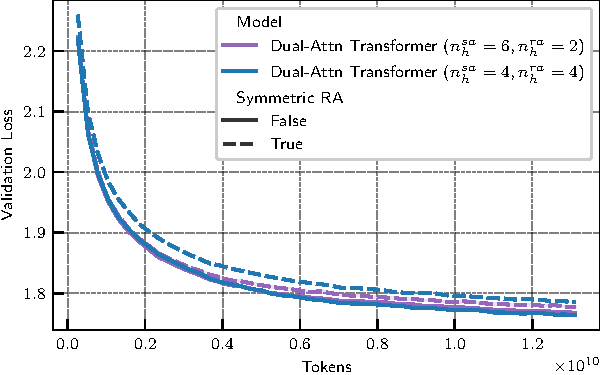
\includegraphics[width=\textwidth]{figs/experiments/tiny_stories/d64L4_ablation_symmetry_posrelsym.pdf}
%         \caption{$d = 64, L = 4$, position-relative symbol assignment}
%     \end{subfigure}
%     \caption{Ablation of Symmetry in relational attention. The \textit{DAT} models with asymmetric relations perform slightly better than those with a symmetry constraint.}\label{fig:ablation_symmetry}
% \end{figure}

% \Cref{tab:tiny_stories_results} shows the end-of-training validation loss and perplexity for all models we evaluated. For each $\dmodel, L$ the best-performing model is bolded. We find that the \textit{DAT} model with asymmetric relational attention and symbolic attention consistently performs the best, beating out the Transformer by a small margin.

% \Cref{fig:ablation_symbol_type} depicts an ablation over symbol type. For $\dmodel = 64, L = 4$, it shows training curves for \textit{DAT} models with two types of symbol retrieval mechanism: symbolic attention and position-relative symbol. We find that the symbolic attention variant learns faster and reaches a smaller loss. This holds both when relational attention uses symmetric or asymmetric relations. We posit the explanation that the differentiable equivalence class mapping implemented by symbolic attention may capture a form of syntax.

% \Cref{fig:ablation_symmetry} shows an ablation over the symmetry of relational attention. Relational attention can be constrained to represent symmetric relations by imposing that $\Wqrel = \Wkrel$. This is sometimes a useful inductive bias, as observed in the relational games experiments. However, in the language modeling experiments, we found that it was not a useful inductive bias and that asymmetric relational attention outperformed symmetric relational attention. One possible explanation is that the types of relations that are relevant in parsing language are in general asymmetric. For example, syntactic or grammatical relations such as noun-verb, subject-object, determiner-noun, etc. are asymmetric.

% \subsection{Image Recognition (Section \ref{ssec:imagenet})}

% \subsubsection*{Experimental details}

% \textbf{Dataset details.} For this experiment, we use the ImageNet Large Scale Visual Recognition Challenge 2012 (ILSVRC2012) dataset~\citep{imagenet}. The dataset is roughly 140GB in size and consists of RGB images hand-labeled with the presence or absence of 1,000 object categories. We train on images resized to $224 \times 224$. In the training set, we perform a random crop and resize to $224 \times 224$, then normalize channel-wise with means $(0.485, 0.456, 0.406)$ and standard deviations $(0.229, 0.224, 0.225)$. For the validation set, we resize to $256 \times 256$ then center crop to $224 \times 224$, and normalize in the same way.

% \textbf{Model architectures.} We use a Vision Transformer-style architecture \citep{dosovitskiyImageWorth16x162020}. ImageNet's $224 \times 224 \times 3$ RGB images are divided into $16 \times 16$ patches, flattened, and linearly embedded into a vector. A learnable positional embedding is added to each patch embedding. We also prepend a special classification token. The sequence of patch embeddings is then fed through an Encoder and the embedding of the class token is used to generate the final classification through a fully connected layer. We compare a Vision Transformer model with $n_h^{sa} = 16$ to an \textit{DAT} model with $n_h^{sa} = 10, n_h^{sa} = 6$. For both, we used a model dimension $\dmodel = 1024$, $L = 24$ layers, MLP hidden dimension $\dff = 4096$, SwiGLU activation, no bias, dropout rate = 0.1, and pre-LayerNormalization. The \textit{DAT} model uses position-relative symbols as the symbol assignment mechanism and symmetric relational attention.

% \textbf{Training details.} Both models are trained with the AdamW optimizer, with a constant learning rate of $5 \times 10^{-4}$ and $\beta_1 = 0.9, \beta_2 = 0.99$. We used a batch size of 32 and 32 gradient accumulation steps.

% \aawarning{TODO -- note that we did not perform any regularization (other than dropout) and did not use any data augmentation. it is likely possible that significant improvements would be possible with additional regularization. In fact,~\citet{dosovitskiyImageWorth16x162020} notes that when trained on medium-sized datasets like ImageNet, strong regularization is required.}